\documentclass[a4paper, 11pt]{article}
\usepackage[utf8]{inputenc}
\usepackage[swedish]{babel}
\usepackage{amsmath}
\usepackage[arrowdel]{physics}
\usepackage{listings}
\usepackage{hyperref}

\newcommand{\Ordo}[1]{\ensuremath{O\left(#1\right)}}
\newcommand{\deval}[4][]{\dv[#1]{#2}{#3} (#4)}
\newcommand{\pdeval}[4][]{\pdv[#1]{#2}{#3} (#4)}
\newcommand{\inteval}[4]{\int\limits_{#1}^{#2}#3\dd{#4}}
\newcommand{\proof}{\subparagraph{Bevis}}
\newcommand{\expec}[1]{\text{E}\left(#1\right)}

\title{Sammanfattning av SF1544 Numeriska metoder, grundkurs}
\author{Yashar Honarmandi \\ yasharh@kth.se}
\date{\today}

\begin{document}

\maketitle

\begin{abstract}
	Detta ær en sammanfattning av kursen SH1014 Modern fysik.
\end{abstract}

\pagenumbering{roman}
\thispagestyle{empty}

\newpage

\tableofcontents

\newpage

\pagenumbering{arabic}

\section{Användbar matte}

\paragraph{Allmän begränsning av globalt fel}
Betrakta begynnelsevärdesproblemet
\begin{align*}
	\deval{y}{t}{t} &= f(t, y(t)), \\
	y(a)            &= b,
\end{align*}
löst på $[a, T]$, där $f$ är Lipschitzkontinuerlig. Betrakta en numerisk lösning med lokalt fel begränsad av $Mh^{p + 1}$. Då begränsas det globala felet av
\begin{align*}
	\abs{y(T) - y_{N}} \leq \frac{e^{L(T - a)}M}{L}h^{p}.
\end{align*}

\proof
Vi inför $y(t; t_{n})$ som den exakta lösningen som startar i $(t_{n}, y_{n})$. Det globala felet ges då av
\begin{align*}
	\abs{y(T) - y_{N}} &= \abs{y(T) - y(T; t_{N - 1}) + y(T; t_{N - 1}) + \dots - y(T; t_{1}) + y(T; t_{1}) - y_{N}} \\
	                   &\leq \abs{y(T) - y(T; t_{N - 1})} + \abs{y(T; t_{N - 1}) - y(T; t_{N - 2})} + \dots + \abs{y(T; t_{1}) - y_{N}}.
\end{align*}
Den första termen ges simpelthen av det lokala felet. Satsen om entydighet av lösning för en sådan differentialekvation ger vidare
\begin{align*}
	\abs{y(T; t_{i}) - y(T; t_{i - 1})} \leq e^{L(T - t_{i})}\abs{y(t_{i}; t_{i}) - y(t_{i}; t_{i - 1})}.
\end{align*}
Det som står kvar i absolutbeloppstecknet är det lokala felet, eftersom den vänstra termen är exakt och den högra kommer från en iteration. Detta ger
\begin{align*}
	\abs{y(T; t_{i}) - y(T; t_{i - 1})} \leq e^{L(T - t_{i})}Mh^{p + 1} = e^{L(N - i)h}Mh^{p + 1}
\end{align*}
och vidare
\begin{align*}
	\abs{y_{N} - y(T)} &\leq Mh^{p + 1} + Mh^{p + 1}e^{Lh} + \dots + Mh^{p + 1}e^{L(N - 1)h}. \\
	                   &= Mh^{p + 1}\frac{1 - e^{LNh}}{1 - e^{Lh}} \\
	                   &= Mh^{p + 1}\frac{e^{LNh} - 1}{e^{Lh} - 1} \\
	                   &\leq Mh^{p + 1}\frac{e^{LNh}}{Lh},
\end{align*}
och beviset är klart.

\paragraph{Möjlighet för polynominterpolation}
Givet $n + 1$ punkter $(x_{i}, y_{i})$, där $x_{i}\neq x_{j}$ om $i\neq j$, finns det ett entydigt polynom $p$ av grad (högst) $n$ så att $p(x_{i}) = y_{i}\ \forall i= 1, \dots, n + 1$.

\proof
För att visa existensen av $p$, kan vi välja det som
\begin{align*}
	p(x) = \sum\limits_{i = 1}^{n + 1}y_{i}\prod\limits_{j\neq i}\frac{x - x_{j}}{x_{i} - x_{j}}.
\end{align*}
Denna metoden kallas för Lagrangeinterpolation. Vi ser att $p$ har grad $n$ och
\begin{align*}
	p(x_{k}) = \sum\limits_{i = 1}^{n + 1}y_{i}\prod\limits_{j\neq i}\frac{x_{k} - x_{j}}{x_{i} - x_{j}}.
\end{align*}
För alla termer i summan där $i\neq k$ kommer det finnas en faktor $x_{k} - x_{k}$ i nämnaren, och dessa ger inget bidrag. För $i = k$ blir produkten bara $1$, och $p(x_{k}) = y_{k}$.

För att visa att $p$ är entydig, antag att $q$ är ett annat interpolationspolynom och bilda $v = q - p$, med grad högst $n$. Detta ger att $v$ har $n + 1$ nollställen. Detta är endast möjligt om $v = 0$, och därmed måste $p$ vara unikt.

\paragraph{Fel för linjär interpolation}
Antag att $f\in C^{2}$. Låt $p$ vara det linjära polynomet som interpolerar punkterna $(x_{0}, f(x_{0})$ och $(x_{0} + h, f(x_{0} + h)$. Då gäller $\abs{f(x) - p(x)} \leq Ch^{2},\ x_{0} \leq x \leq x_{0} + h$, där
\begin{align*}
	C = \max\limits_{x_{0} \leq z \leq x_{0} + h}\frac{\abs{\deval[2]{f}{x}{z}}}{8}.
\end{align*}

\proof
Antag $x_{0} = 0$, och bilda $g = f - p$. $g$ är kontinuerlig på $[0, h]$, och antar därmed ett största och minsta värde på detta intervallet. Antag att den antar sitt största värde i $x = a$. Taylorutveckling kring $a$ ger
\begin{align*}
	g(x) = g(a) + \deval{g}{x}{a}(x - a) + \frac{1}{2}\deval[2]{g}{x}{c}(x - a)^{2}
\end{align*}
för något $c\in [a, x]$. Vi ser att andra termen måstse bli $0$, ty $a$ är en maxpunkt. Evaluering av Taylorutvecklingen i $x = 0$ eller $x = h$ (den som är närmast $a$) ger $g(x) = 0$ och
\begin{align*}
	g(a)       &= -\frac{1}{2}\deval[2]{g}{x}{c}(x - a)^{2},
	\abs{g(a)} &\leq \frac{1}{2}\max\limits_{x_{0} \leq z \leq x_{0} + h}\abs{\deval[2]{g}{x}{z}}\left(\frac{1}{2}h\right)^{2}.
\end{align*}
Vi vet att $\deval[2]{f}{x}{x} = \deval[2]{g}{x}{x}$ eftersom $p$ är linjär, vilket ger
\begin{align*}
	\abs{g(a)} &\leq \max\limits_{x_{0} \leq z \leq x_{0} + h}\frac{\abs{\deval[2]{f}{x}{z}}}{8}h^{2}.
\end{align*}

\paragraph{Konvergens för potensmetoden}
Antag för en given matris $A$ att dens egenvärden uppfyller $\abs{\lambda_{1}} > \abs{\lambda_{2}} \geq \dots \geq \abs{\lambda_{n}}$ och att dens egenvektorer $v_{1}, \dots, v_{n}$ spänner upp $\R^{n}$. Då konvergerar potensmetoden för nästan alla startvektorer $x^{0}$ till egenvektorn $v_{1}$ och egenvärdet $\lambda_{1}$, med maximal konvergensrate $\abs{\frac{\lambda_{2}}{\lambda_{1}}}$.

\proof
Vi kan skriva
\begin{align*}
	x^{0} = \sum\limits_{i = 1}^{n}c_{i}v_{i}.
\end{align*}
Om $c_{1} \neq 0$ ger $k$ multiplikationer med $A$
\begin{align*}
	A^{k}x^{0} = \sum\limits_{i = 1}^{n}\lambda_{i}^{k}c_{i}v_{i}.
\end{align*}
Potensmetoden ger oss nu
\begin{align*}
	x^{k + 1} = \frac{1}{\norm{\sum\limits_{i = 1}^{n}\lambda_{i}^{k}c_{i}v_{i}}}\sum\limits_{i = 1}^{n}\lambda_{i}^{k}c_{i}v_{i}.
\end{align*}
Om vi antar att både $c_{1}$ och $\lambda_{1}$ är positiva, kan detta skrivas som
\begin{align*}
	x^{k + 1} = \frac{1}{\norm{\sum\limits_{i = 1}^{n}\left(\frac{\lambda_{i}}{\lambda_{1}}\right)^{k}\frac{c_{i}}{c_{1}}v_{i}}}\sum\limits_{i = 1}^{n}\left(\frac{\lambda_{i}}{\lambda_{1}}\right)^{k}\frac{c_{i}}{c_{1}}v_{i}.
\end{align*}
Om $\lambda_{1}$ är negativ, kan man dividera med dens belopp. Om $c_{1}$ är negativ, får du fortfarande konvergens mot en egenvektor motsvarande egenvärdet $\lambda_{1}$.

Enligt antagandet kommer iterationen för stora $k$ att konvergera mot $\frac{v_{1}}{\norm{v_{1}}}$. Vi noterar även att enligt antagandet är det termen motsvarande $i = 2$ som konvergerar långsammast, och att konvergensen sker med en faktor $\abs{\frac{\lambda_{2}}{\lambda_{1}}}$.

\section{Grundläggande definitioner och analys}

\paragraph{Krafter på en stång}
Betrakta en stång med tvärsnittsarea $A$ som utsätts för en kraft $P$ i varje ända, med motsatt riktning i varje ända, som visad i figur \ref{fig:cylinder_forces}.
\begin{figure}[!ht]
	\centering
	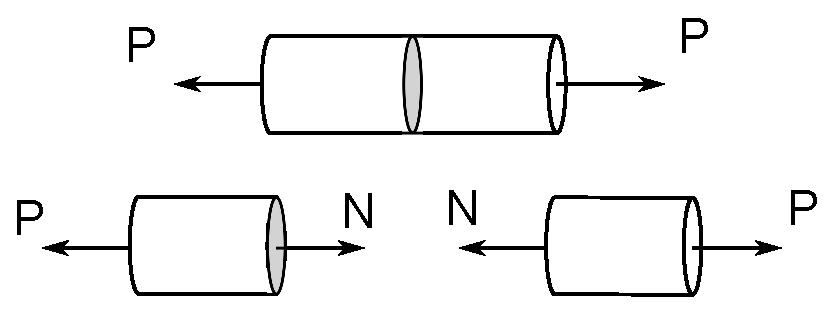
\includegraphics[width = 0.5\textwidth]{./Images/cylinder_forces.eps}
	\caption{Illustration av en stång som utsätts för en dragkraft och de orsakade inre krafterna.}
	\label{fig:cylinder_forces}
\end{figure}

Kraften $P$ i änderna propageras som inre krafter i stången. Om vi betraktar det indikerade tvärsnittet, manifesteras den inre kraften som en normalkraft på varje halva. Om vi definierar positiv riktning för normalkraften och dragkraften som i figuren, ger kraftjämvikten att $N = P$.

Om dragkraften blir en tryckkraft, ändrar givetvis normalkraften riktning. Detta kommer inte nödvändigtvis fram av kraftjämvikten. Därför väljer vi konventionen att normalkrafter alltid pekar ut från ytan. Då skulle kraftjämvikten för en pålagd tryckkraft bli $P = -N$, och vi ser att dragkrafter ger positiva normalkrafter och tryckkrafter negativa.

\paragraph{Statiskt bestämta och obestämta problem}
Ett problemt är statiskt bestämt om alla inre krafter och reaktionskrafter kan bestämmas enbart med jämvikt. Detta är möjligt om det verkar maximalt $3$ krafter i planet eller $6$ i rymden.

Om ett problem ej är statiskt bestämt, är det statiskt obestämt. Då räcker icke jämviktsekvationerna, och det motsvarar (ofta) att man kan ta bort ett element och vara kvar i jämvikt. För att lösa statiskt obestämda problem behövs typiskt materialsamband från hållfasthetsläran.

\paragraph{Spänning}
I hållfasthetslära är vi intresserade av påkänningen på materialet. Den beror av beloppet av normalkraften, men kan även spridas ut över tvärsnittet. Därför definierar vi spänningen
\begin{align*}
	\sigma = \frac{N}{A}.
\end{align*}
Jämvikten från innan ger
\begin{align*}
	\sigma = \frac{P}{A}.
\end{align*}

\paragraph{Deformation}
När en stång utsätts för spänning, kommer den att deformeras. Eftersom förlängningen av varje del kommer från kraftjämvikten mellan normalkraften och dragkraften, kommer förlängningen för en given dragkraft bero av längden. Vi definierar därför töjningen
\begin{align*}
	\varepsilon	= \frac{\delta}{L_{0}}
\end{align*}
där $L_{0}$ är stångens ursprungliga längd och $\delta$ är förlängningen.

\paragraph{Typer av samband i hållfasthetslära}
I hållfasthetsläran har vi tre typer av samband:
\begin{itemize}
	\item samband mellan krafter.
	\item samband mellan deformationer.
	\item konstitutiva samband (beskrivar materialbeteende).
\end{itemize}

\paragraph{Hookes lag}
Om man gör dragningsprov på olika material för små deformationer, blir plottet av $\sigma$ mot $\varepsilon$ approximativt linjär. Från detta får vi Hookes lag:
\begin{align*}
	\sigma = E\varepsilon.
\end{align*}
$E$ är elasticitetsmodulen, och beskrivar hur styvt materialet är.

Kombinationen av det vi har tills nu ger
\begin{align*}
	P = \frac{EA}{L}\delta
\end{align*}
för en homogen stång som utsätts för en dragkraft $P$.

Om ett material komprimeras, visar det sig att det elastiska beteendet ofta är likt, med samma elasticitetsmodul.

\paragraph{Normalspänning}
Vi utvidgar våran definition av spänning till spänningar som fördelas inhomogent över tvärsnittet vid att betrakta en inre kraft $\Delta F$ som verkar på ett arealement $\Delta A$, med riktningar som tidigare. Då definieras normalspänningen som
\begin{align*}
	\sigma = \lim\limits_{\Delta A\to 0}\frac{\Delta F}{\Delta A}.
\end{align*}

\paragraph{Normaltöjning}
Vi utvidgar även definitionen av töjning till töjningar som fördelas ojämnt över stavens längd. Om deformationen i en punkt är $u(x)$, ges töjningen av ett litet element med längd $\Delta x$ av
\begin{align*}
	\varepsilon = \lim\limits_{\Delta x\to 0}\frac{u(x + \Delta x) - u(x)}{\Delta x} = \dv{u}{x}.
\end{align*}
Vi ser av detta att töjningen är linjär, så vi kan addera bidrag till den.

\paragraph{Termoelasticitet}
Låt $T$ beteckna en stångs temperatur. En temperaturändring orsakar en termisk töjning
\begin{align*}
	\varepsilon_{T} = \alpha\Delta T,
\end{align*}
där $\alpha$ är längdutvidgningskoefficienten. Man behöver givetvis utgå från en referenstemperatur.

\paragraph{Allmänt enaxligt tillstånd}
Från det vi har sett hittils, kan vi skriva upp en differentialekvation som beskriver det enaxliga tillståndet.

Betrakta en stång med variabel tvärsnittsyta där det överallt i kroppen verkar en volymskraft $K(x)$ (kraft per volym), samt krafter $P_{\text{V}}$ respektiva $P_{\text{H}}$ i varje ända. Vi betraktar ett litet element med tjocklek $\dd{x}$. I ena ändan verkar kraften $K(x)A\dd{x}$ och en normalkraft $N(x)$ på grund av krafterna på volymelementet till vänster, och i andra ändan verkar en normalkraft $N(x + \dd{x})$ på grund av krafterna på volyemelementet till höger.

Kraftjämvikten ger
\begin{align*}
	N(x + \dd{x}) - N(x) + K(x)A\dd{x} &= 0, \\
	\dd{N}{x} + K(x)                   &= 0.
\end{align*}
Vi inför nu definitionen av töjninc och skriver den som en linjärkombination av bidrag från spänning och termoelasticitet, vilket ger
\begin{align*}
	\varepsilon = \frac{\sigma}{E} + \alpha\Delta T, \\
	\sigma = E(\varepsilon - \alpha\Delta T).
\end{align*}
Kombinerad med definitionen av töjning ger det
\begin{align*}
	\dv{x} (\sigma A) + K(x)A &= 0, \\
	\dv{x} (EA(\varepsilon - \alpha\Delta T)) + K(x)A &= 0, \\
	\dv{x}\left(EA\dv{u}{x}\right) + K(x)A &= \dv{x}(EA\alpha\Delta T).
\end{align*}
Detta kommer med randvillkor, och är typiskt randvillkor i deformationen eller i spänningen. Eftersom spänningen är proportionell mot derivatan av deformationen, motsvarar dessa Dirichlet- respektiva Neumannvillkor.

\paragraph{Tvärkontraktion}
När man gör ett dragningsprov på en kropp, genomgår den deformation i längdriktning samtidigt som tjockleken minskar. Detta kallas tvärkontraktion. Töjningen $\varepsilon_{t}$ av tjockleken är relaterad till töjningen i längdriktning genom
\begin{align*}
	\varepsilon_{t} = -\nu\varepsilon,
\end{align*}
där $\nu$ är Poissons konstant. Termodynamiken ger att $-1\leq\nu\leq 0.5$.

\paragraph{Skjuvspänning}
Betrakta två plattor som ligger på varandra och dras åt motsatta håll av en kraft $F$ på varje. Om de inte dras isär, balanseras dragkrafterna av krafter i kontaktytan. Låt $A$ vara kontaktytan mellan plattorna. Då definieras skjuvspänningen som
\begin{align*}
	\tau = \frac{F}{A}.
\end{align*}

\paragraph{Deformation från skjuvkrafter}
Betrakta ett rätblock med basarea $A$ och höjd $H$ som dras av motsatt riktade krafter med belopp $F$ på varje sida, illustrerad i figur \ref{fig:rectangle_twist}.
\begin{figure}[!ht]
	\centering
	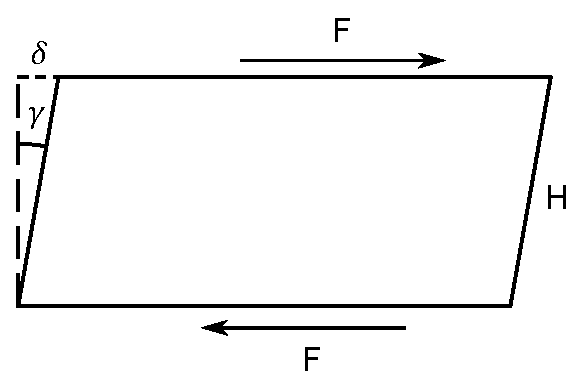
\includegraphics[width = 0.5\textwidth]{./Images/rectangle_twist.eps}
	\label{fig:rectangle_twist}
\end{figure}

Vi kan här definiera skjuvspänningen som
\begin{align*}
	\tau = \frac{F}{A},
\end{align*}
då vi kan tänka oss att plattorna som dras isär är tunna skikt i materialet. Skjuvkrafterna kommer skapa en deformation $\delta$ på en sida motsvarande vridning med en vinkel $\gamma$. Denna vinkeln uppfyller
\begin{align*}
	\tan{\gamma} = \frac{\delta}{H}.
\end{align*}
För små deformationer kan vi approximera
\begin{align*}
	\gamma = \frac{\delta}{H}.
\end{align*}
Experimentellt har man sett att
\begin{align*}
	\tau = G\gamma,
\end{align*}
där $G$ är skjuvmodulen.

\paragraph{Samband mellan materialstorheter}
För ett isotropt material gäller att
\begin{align*}
	G = \frac{E}{2(1 + \nu)}.
\end{align*}

\paragraph{Spänning}
Vi definierar spänningsvektorn
\begin{align*}
	\vb{s} = \lim\limits_{A \to 0}\frac{\vb{F}}{A}
\end{align*}
där $\vb{F}$ är kraften på det lilla arealementet. Den har en komponent normalt på ytan, som är normalspänningen, och en komponent som är parallel med ytan, som är skjuvspänningen. Vi får
\begin{align*}
	\sigma = \vb{s}\cdot\vb{n}, \tau^{2} = \abs{\vb{s}}^{2} - \sigma^{2}.
\end{align*}

\paragraph{Skjuvspänningar i tre dimensioner}
Snitta nu ut en infinitesimal kub. På ytorna, till exempel ytan som är normal på $x$-axeln, kan man dekomponera spänningsvektorn i en normalspänning $\sigma_{x}$ och två skjuvspänningar $\tau_{xy}, \tau_{xz}$, och motsvarande i andra riktningar. Om vi tittar på momentjämvikt kring kubens centrum i $x$-riktning fås
\begin{align*}
	2\tau_{yz}\dd{x}\dd{z}\cdot\frac{1}{2}\dd{y} - 2\tau_{zy}\dd{x}\dd{y}\cdot\frac{1}{2}\dd{z}        &= 0, \\
	\tau_{yz} &= \tau_{zy}.
\end{align*}
En motsvarande härledning kan göras för de andra sidorna. Tillkommer det andra termer om skjuvspänningen varierar? Ja, men dessa kommer vara av högre ordning, och kan försummas.

\paragraph{Spänningsmatris}
Vi kan nu definiera en spänningsmatris
\begin{align*}
	S =
	\mqty[
		\sigma_{x} & \tau_{yx}  & \tau_{zx} \\
		\tau_{xy}  & \sigma_{y} & \tau_{zy} \\
		\tau_{xz}  & \tau_{yz}  & \sigma_{z}
	].
\end{align*}
Enligt argumentet ovan är denna symmetrisk.

\paragraph{Spänningar på godtycklig yta}
Om man har en godtycklig yta med normalvektor $\vb{n}$, kan det visas att spänningarna på ytan ges av
\begin{align*}
	\vb{s} = S\vb{n}.
\end{align*}
Vi kan då skriva
\begin{align*}
	\sigma &= \vb{n}^{T}S\vb{n}, \\
	\tau   &= \abs{S\vb{n}}^{2} - (\vb{n}^{T}S\vb{n})^{2}.
\end{align*}

\paragraph{Huvudspänningar}
Finns det orienteringar sådana att $\vb{s} = \sigma\vb{n}$? Att hitta sådana är ett egenvärdesproblem. Matematiken ger att det finns sådana orienteringar, och att de är ortogonala mot varandra.

Beteckna även den största respektiva minsta huvudspänningen som $\sigma_{1}$ respektiva $\sigma_{3}$. Då ges den maximala skjuvspänningen i materialet av
\begin{align*}
	\tau_{\text{max}} = \frac{\sigma_{1} - \sigma_{3}}{2}.
\end{align*}

\paragraph{Plana tillstånd}
Ett specialfall är när $z$-riktningen är en huvudriktning för spänningen. Då är skjuvspänningarna i $xy$-planet, dvs. $\tau_{zx} = \tau_{zy} = 0$. Om $\sigma_{z} = 0$, har man plan spänning.

Betrakta plan spänning på ett plan som bildar en vinkel $\phi$ med $y$-axeln. Normalvektorn ges av
\begin{align*}
	\vb{n} = \cos{\phi}\vb{e}_{x} + \sin{\phi}\vb{e}_{y}.
\end{align*}
Vi får då
\begin{align*}
	\sigma &= \sigma_{x}\cos[2]{\phi} + \sigma_{y}\sin[2]{\phi} + 2\tau_{xy}\sin{\phi}\cos{\phi}, \\
	\tau   &= \tau_{xy}\cos{2\phi} + \frac{\sigma_{y} - \sigma_{x}}{2}\sin{2\phi}.
\end{align*}

\paragraph{Mohrs spänningscirkel}
Mohrs spänningscirkel är ett sätt att grafiskt ta fram plana spänningar vid rotation av ett plan. För att konstruera cirkeln, rita upp ett $\sigma, \tau$-koordinatsystem och två punkter $(sigma_{x}, \tau_{x, y})$ och $(sigma_{y}, -\tau_{x, y})$, där dessa tas från något givet tillstånd. Dessa punkter skall vara i motstående änder av cirkeln, och från detta kan cirkeln ritas, som i figur \ref{fig:mohr_stress_circle}.

\begin{figure}[!ht]
	\centering
	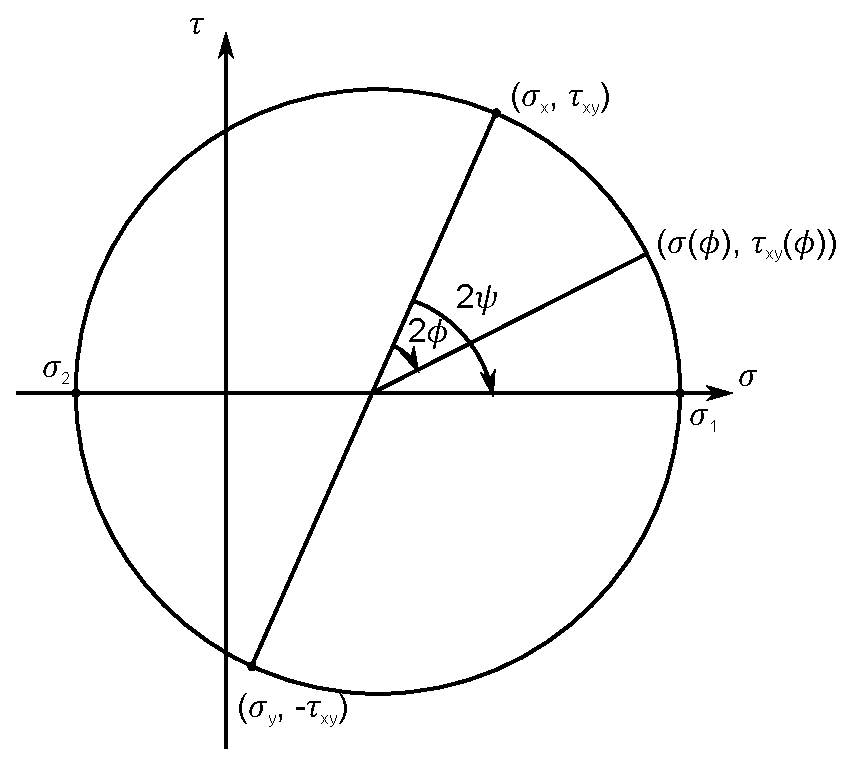
\includegraphics[width = 0.5\textwidth]{./Images/mohr_stress_circle.eps}
	\caption{Mohrs spänningscirkel.}
	\label{fig:mohr_stress_circle}
\end{figure}

En rotation moturs av koordinatsystemet med en vinkel $\phi$ motsvarar en rotation medurs av tillståndet på cirkeln med en vinkel $2\phi$.

Det visar sig att cirkeln skär $\sigma$-axeln i största och minsta huvudspänningen. Det finns även en vinkel $\psi$ som koordinatsystemet måste roteras med så att det blir parallellt med huvudriktningarna. Ur denna geometrin kan vi få följande samband, som är helt konsekventa med tensorbetraktningen gjort ovan:
\begin{align*}
	\sigma_{1}        &= \frac{\sigma_{x} + \sigma_{y}}{2} + \sqrt{\left(\frac{\sigma_{x} - \sigma_{y}}{2}\right)^{2} + \tau_{xy}^{2}}, \\
	\sigma_{2}        &= \frac{\sigma_{x} + \sigma_{y}}{2} - \sqrt{\left(\frac{\sigma_{x} - \sigma_{y}}{2}\right)^{2} + \tau_{xy}^{2}}, \\
	\tan(2\psi)       &= \frac{2\tau_{xy}}{\sigma_{x} - \sigma_{y}}, \\
	\tau_{\text{max}} &= \frac{\sigma_{1} - \sigma_{3}}{2}.
\end{align*}

\paragraph{Jämvikt i tre dimensioner}
Snitta ut en liten kub. Jämvikt i $x$-riktning ger
\begin{align*}
	\sigma(\vb{x} + \dd{x}\vb{e}_{x})\dd{y}\dd{z} - \sigma(\vb{x})\dd{y}\dd{z} + \tau_{zx}(\vb{x} + \dd{z}\vb{e}_{z})\dd{x}\dd{y} - \tau_{zx}(\vb{x})\dd{x}\dd{y} + \tau_{yx}(\vb{x} + \dd{y}\vb{e}_{y})\dd{x}\dd{z} - \tau_{yx}(\vb{x})\dd{x}\dd{z} = 0,
\end{align*}
vilket implicerar
\begin{align*}
	\del{x}{\sigma_{x}} + \del{y}{\tau_{xy}} + \del{z}{\tau_{zx}} = 0.
\end{align*}
På motsvarande sätt fås
\begin{align*}
	\del{x}{\tau_{xy}} + \del{y}{\sigma_{y}} + \del{z}{\tau_{yz}} &= 0, \\
	\del{y}{\tau_{xz}} + \del{y}{\tau_{yz}} + \del{z}{\sigma_{z}} &= 0.
\end{align*}
Om det finns volymkrafter i kroppen, dyker den även upp som en term här.

\paragraph{Töjning i tre dimensioner}
I tre dimensioner definieras töjningen i termer av båglängden som
\begin{align*}
	\varepsilon = \frac{\dd{s} - \dd{s_{0}}}{\dd{s_{0}}},
\end{align*}
där $\dd{s_{0}}$ är den odeformerade båglängden och $\dd{s}$ är den deformerade båglängden.

\paragraph{Tredimensionellt samband mellan töjning och deformation}
Betrakta en kropp som deformeras med en deformationsvektor $\vb{u}$. Snitta ut en kub och titta på två hörn i positioner $x$ och $x + \dv{x}$, med övriga koordinater lika. I det odeformerade läget är avståndet mellan dessa $\dd{s_{0}} = \dd{x}$. I det deformerade läget är avståndet
\begin{align*}
	\dd{s} &= (x + \dd{x} + u_{x}(x + \dd{x}, y, z)) - (x + u_{x}(x, y, z)) \\
	       &= \dd{x} + u_{x}(x + \dd{x}, y, z) - u_{x}(x, y, z) \\
	       &= \dd{x} + \dv{u_{x}}{x}\dd{x},
\end{align*}
och töjningen i $x$-riktning ges av
\begin{align*}
	\varepsilon_{x} = \del{x}{u_{x}}.
\end{align*}
På samma sätt fås
\begin{align*}
	\varepsilon_{y} = \del{y}{u_{y}}, \varepsilon_{z} = \del{z}{u_{z}}.
\end{align*}

\paragraph{Skjuvdeformation i tre dimensioner}
Betrakta en kub som deformeras i $xy$-planet. Sidan närmast $x$-axeln bildar vinkeln $\beta$ med $x$-axeln och sidan närmast $y$-axeln bildar vinkeln $\alpha$ med $y$-axeln. Den totala skjuvvinkeln ges av $\gamma_{yx} = \alpha + \beta$. Geometrin ger
\begin{align*}
	\gamma_{xy} = \frac{u_{x}(x, y + \dd{y}, z) - u_{x}(x, y, z)}{\dd{y}} + \frac{u_{y}(x + dd{x}, y, z) - u_{x}(x, y, z)}{\dd{x}} = \del{y}{u_{x}} + \del{x}{u_{y}}.
\end{align*}
på motsvarande sätt fås
\begin{align*}
	\gamma_{yz} = \del{z}{u_{y}} + \del{y}{u_{z}}, \gamma_{xz} = \del{z}{u_{x}} + \del{x}{u_{z}}.
\end{align*}

\paragraph{Töjningsmatrisen}
Vi definierar töjningsmatrisen
\begin{align*}
	T =
	\mqty[
		\varepsilon_{x}  & \varepsilon_{yx} & \varepsilon_{zx} \\
		\varepsilon_{xy} & \varepsilon_{y}  & \varepsilon_{zy} \\
		\varepsilon_{xz} & \varepsilon_{yz} & \varepsilon_{z}
	],
\end{align*}
där vi inför $\varepsilon_{xy} = \varepsilon_{yx} = \frac{1}{2}\gamma_{xy}$. Detta medför att $T$ är symmetrisk. Det gäller att töjningen i riktningen $\vb{n}$ ges av
\begin{align*}
	\varepsilon_{\vb{n}} = \vb{n}^{T}T\vb{n}.
\end{align*}

\paragraph{Huvudtöjningar}
Finns det orienteringar sådana att $T\vb{n} = \varepsilon\vb{n}$? Att hitta sådana är ett egenvärdesproblem. Matematiken ger att det finns sådana orienteringar, och att de är ortogonala mot varandra.

Beteckna även den största respektiva näst största huvudtöjningen som $\varepsilon_{1}$ respektiva $\varepsilon_{2}$. Då ges den maximala skjuvvinkeln i materialet av
\begin{align*}
	\gamma_{\text{max}} = \varepsilon_{1} - \varepsilon_{2}.
\end{align*}

\paragraph{Mohrs töjningscirkel}
Mohrs töjningscirkel är ett sätt att grafiskt ta fram plana töjningar vid rotation av ett plan. För att konstruera cirkeln, rita upp ett $\varepsilon, \frac{\gamma}{2}$-koordinatsystem och två punkter $(\varepsilon_{x}, \frac{\gamma_{x, y}}{2})$ och $(\varepsilon_{y}, -\frac{\gamma_{x, y}}{2})$, där dessa tas från något givet tillstånd. Dessa punkter skall vara i motstående änder av cirkeln, och från detta kan cirkeln ritas, som i figur \ref{fig:mohr_strain_circle}.

\begin{figure}[!ht]
	\centering
	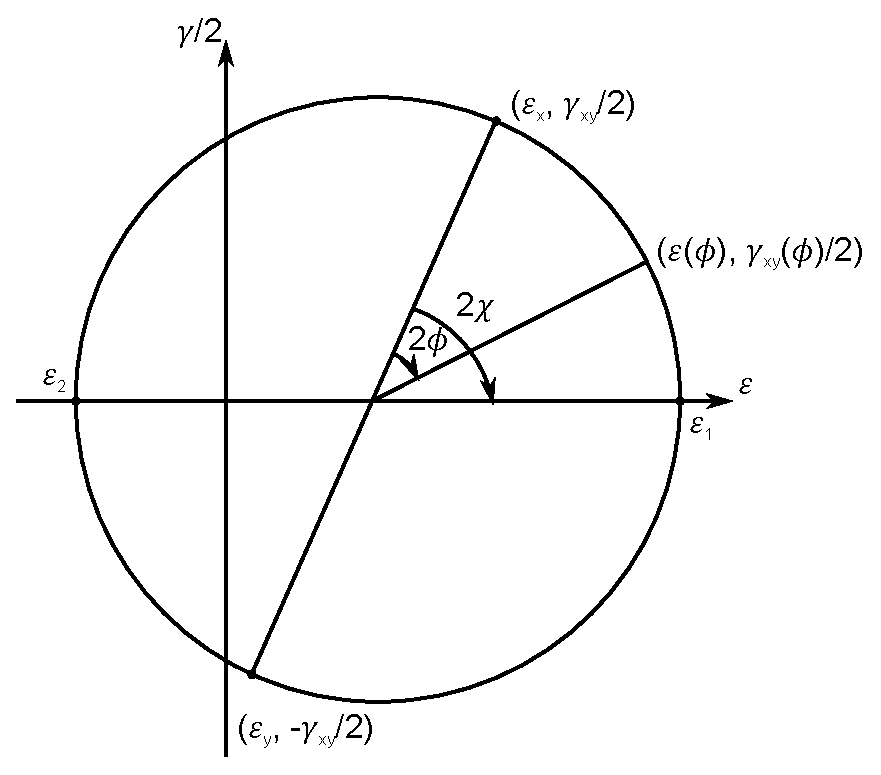
\includegraphics[width = 0.5\textwidth]{./Images/mohr_strain_circle.eps}
	\caption{Mohrs töjningscirkel.}
	\label{fig:mohr_strain_circle}
\end{figure}

En rotation moturs av planet med en vinkel $\phi$ motsvarar en rotation medurs av tillståndet på cirkeln med en vinkel $2\phi$.

Det visar sig att cirkeln skär $\varepsilon$-axeln i största och näst största huvudtöjningen. Det finns även en vinkel $\chi$ som koordinatsystemet måste roteras med så att det blir parallellt med huvudriktningarna. Ur denna geometrin kan vi få följande samband, som är helt konsekventa med tensorbetraktningen gjort ovan:
\begin{align*}
	\varepsilon_{1}     &= \frac{\varepsilon_{x} + \varepsilon_{y}}{2} + \sqrt{\left(\frac{\varepsilon_{x} - \varepsilon_{y}}{2}\right)^{2} + \left(\frac{\gamma_{xy}}{2}\right)^{2}}, \\
	\varepsilon_{2}     &= \frac{\varepsilon_{x} + \varepsilon_{y}}{2} - \sqrt{\left(\frac{\varepsilon_{x} - \varepsilon_{y}}{2}\right)^{2} + \left(\frac{\gamma_{xy}}{2}\right)^{2}}, \\
	\tan(2\psi)         &= \frac{\gamma_{xy}}{\varepsilon_{x} - \varepsilon_{y}}, \\
	\gamma_{\text{max}} &= \varepsilon_{1} - \varepsilon_{2}.
\end{align*}

\paragraph{Kompatibilitet i tre dimensioner}
Från definitionerna av elementerna i töjningsmatrisen kan man se att det gäller att
\begin{align*}
	2\del{x}{\del{y}{\varepsilon_{xy}}} &= \del[2]{y}{\varepsilon_{x}} + \del[2]{x}{\varepsilon_{y}}, \\
	2\del{y}{\del{z}{\varepsilon_{yz}}} &= \del[2]{z}{\varepsilon_{y}} + \del[2]{y}{\varepsilon_{z}}, \\
	2\del{z}{\del{x}{\varepsilon_{zx}}} &= \del[2]{x}{\varepsilon_{z}} + \del[2]{z}{\varepsilon_{x}}.
\end{align*}
Alltså är inte de olika töjningarna oberoende.

\paragraph{Linjärelastiska material}
I linjärelastiska material gäller sambandet $S = CT$, där $C$ är en fjärde ordningens tensor. Detta kan alternativt skrivas som $T = C^{-1}S$.

\paragraph{Hookes lag för isotropa material}
I isotropa material är alla riktningar lika. I dessa materialer gäller Hookes lag
\begin{align*}
	\varepsilon_{x} &= \frac{1}{E}(\sigma_{x} - \nu(\sigma_{y} + \sigma_{z})) + \alpha\Delta T, \\
	\varepsilon_{y} &= \frac{1}{E}(\sigma_{y} - \nu(\sigma_{x} + \sigma_{z})) + \alpha\Delta T, \\
	\varepsilon_{z} &= \frac{1}{E}(\sigma_{z} - \nu(\sigma_{x} + \sigma_{y})) + \alpha\Delta T, \\
	\gamma_{xy}     &= \frac{1}{G}\tau_{xy}, \\
	\gamma_{yz}     &= \frac{1}{G}\tau_{yz}, \\
	\gamma_{xz}     &= \frac{1}{G}\tau_{xz},
\end{align*}
där $E$ är elasticitetsmodulen, $G$ är skjuvmodulen och $\nu$ är Poissons tal.

\paragraph{Samband mellan elasticitetsmodul och skjuvmodul}
Betrakta ett plant skjuvtillstånd med skjuvspänning $\tau_{xy}$ för ett isotropt material. Med Moores spänningscirkel fås huvudspänningarna $\sigma_{1} = \tau_{xy}, \sigma_{2} = -\tau_{xy}$. Hookes lag ger
\begin{align*}
	\varepsilon_{1} = \frac{1 + \nu}{E}\tau_{xy}, \varepsilon_{2} = -\frac{1 + \nu}{E}\tau_{xy}.
\end{align*}
Mohrs töjningscirkel ger vidare
\begin{align*}
	\frac{\gamma_{xy}}{2} = \varepsilon_{1} = \frac{1 + \nu}{E}\tau_{xy}.
\end{align*}
Jämförelse med Hookes lag ger
\begin{align*}
	G = \frac{1}{2(1 + \nu)}E.
\end{align*}

\paragraph{Tunnväggiga tryckkärl}
Betrakta ett cylindrikskt tryckkärl med innerradie $a$ och väggtjocklek $h$ med ett inre tryck $p$. Vi kommer studera detta i cylindriska koordinater.

Det finns spänningar $\sigma_{z}$ och $\sigma_{\phi}$ i tryckkärlet. Cylindersymmetrin ger att båda dessa är oberoende av $\phi$. Det återstår bara att använda jämvikter för att beräkna dem.

Snitta nu ut en halvcylindrisk del med längd $\Delta z$, detta för att ej behöva betrakta radiella spänningar. Kraftjämvikt på ytan vi snittar genom ger
\begin{align*}
	2a\Delta zp - 2h\Delta z\sigma_{\phi} &= 0, \\
	\sigma_{\phi}                         &= \frac{pa}{h}.
\end{align*}

Snitta nu normalt på $z$-axeln. Om vi försummar kraftbidrag från annat än trycket i kärlet, ger kraftjämvikten
\begin{align*}
	2\pi ah\sigma_{z} - \pi a^{2}p &= 0, \\
	\sigma_{z}                     &= \frac{pa}{2h}.
\end{align*}

Om man tittar i radiell riktning, har vi randvillkoret $\sigma_{r} = -p$ på inre delen av mantelytan. Detta värdet är mycket mindre än de två andra spänningarna, så för tunnväggiga kärl approximerar vi $\sigma_{r} = 0.$

Vi får även töjningar av detta trycket. Om vi får en radiell töjning $u_{r}$, får vi en töjning $2\pi u_{r}$ i $\phi$-riktning.

Man kan göra samma beräkningar för ett sfäriskt kärl, och får
\begin{align*}
	\sigma_{\theta} = \sigma_{\phi} = \frac{pa}{2h}, \sigma_{r} = 0.
\end{align*}
Töjningarna ges av
\begin{align*}
	u_{\theta} = u_{\phi} = 2\pi u_{r}.
\end{align*}

\paragraph{Tjockväggiga tryckkärl}
Betrakta återigen ett cylindriskt tryckkärl, denna gången med innerradie $a$ och ytterradie $b$.

Snitta återigen normalt på $z$-axeln. Detta ger
\begin{align*}
	\sigma_{z} = \frac{pa^{2}}{b^{2} - a^{2}}.
\end{align*}

Snitta nu ut en bit av kärlet med vinkelbrädd $\Delta\phi$, höjd $\Delta z$ och tjocklek $\Delta r$. Vi har spänningar på alla sidor. Geometrin ger att spänningarna i $\phi$-riktning bildar vinkeln $\frac{\Delta\phi}{2}$ med den radiella normalen. Jämvikt i radiell riktning ger då
\begin{align*}
	(r + \Delta r)\Delta\phi\Delta z\sigma_{r}(r + \Delta r) - r\Delta\phi\Delta z\sigma_{r}(r) - 2\frac{\Delta\phi}{2}\Delta z\Delta r\sigma_{\phi} = 0.
\end{align*}
Detta kan lösas för att ge
\begin{align*}
	\frac{(r + \Delta r)\sigma_{r}(r + \Delta r) - r\sigma_{r}(r)}{\Delta r} - \sigma_{\phi} = 0,
\end{align*}
vilket i gränsen ger
\begin{align*}
	\dv{r}(r\sigma_{r}) - \sigma_{\phi} = 0.
\end{align*}

Notera att det ligger bakom att vissa skjuvspänningar blir $0$ för dena sortens symmetri.

Betrakta vidare deformationen och töjningarna. Vi får i radiell riktning
\begin{align*}
	\varepsilon_{r} = \frac{\Delta r + u_{r}(r + \Delta r) - u_{r}(r) - \Delta r}{\Delta r} \to\dv{u_{r}}{r}
\end{align*}
och i vinkelriktning
\begin{align*}
	\varepsilon_{\phi} = \frac{(r + u_{r})\Delta\phi - r\Delta\phi}{r\Delta\phi} = \frac{u_{r}}{r}.
\end{align*}
Vi kan kombinera dessa ekvationerna med Hookes lag för att få
\begin{align*}
	\dv{r}(r^{3}\dv{\sigma_{r}}{r}) = 0.
\end{align*}
På inre randen har vi
\begin{align*}
	\sigma_{r}(a) = -p.
\end{align*}
Om vi har en yttre last $q$, har vi även randvillkoret
\begin{align*}
	\sigma_{r}(a) = -q.
\end{align*}
Detta kan kombineras till att ge
\begin{align*}
	\sigma_{r}    &= \frac{p - \left(\frac{b}{a}\right)^{2}q}{\left(\frac{b}{a}\right)^{2} - 1} - \frac{p - q}{\left(\frac{b}{a}\right)^{2} - 1}\frac{b^{2}}{r^{2}}, \\
	\sigma_{\phi} &= \frac{p - \left(\frac{b}{a}\right)^{2}q}{\left(\frac{b}{a}\right)^{2} + 1} - \frac{p - q}{\left(\frac{b}{a}\right)^{2} - 1}\frac{b^{2}}{r^{2}}.
\end{align*}

\section{Lösning av ekvationer}

\paragraph{Fixpunktsmetoden}
Betrakta ekvationen
\begin{align*}
	x = g(x).
\end{align*}

Fixpunktsmetoden är en enkel iterationsmetod för att lösa denna ekvationen, med den enkla iterationsformeln
\begin{align*}
	x_{n + 1} = g(x_{n}).
\end{align*}

En pseudokod-beskrivning av en lösning med startvillkor \verb|x0| där det itereras tills lösningen stämmer med en tolerans \verb|t| är:
\begin{lstlisting}
	define g(x)
	input x0
	input t
	while abs(x - g(x)) > t
		x = g(x)
	end
	return x
\end{lstlisting}

\subparagraph{Konvergens}
Om $g\in C^{1}$, $\abs{\deval{g}{x}{\alpha}} < 1$ och $\alpha$ är en fixpunkt. finns det en omgivning till $\alpha$ så att om $x_{0}$ är i denna omgivningen, går $x_{n}\to\alpha$. Metoden konvergerar linjärt med reduktionsfaktor $S = \abs{\deval{g}{x}{\alpha}}$.

För att visa detta, skriver vi
\begin{align*}
	x_{n + 1} - \alpha = g(x_{n}) - g(\alpha) = \deval{g}{x}{c}(x_{n} - \alpha),
\end{align*}
där vi har användt medelvärdesatsen och det faktum att $\alpha$ är en fixpunkt. Vidare, eftersom $g\in C^{1}$ finns det en omgivning till $\alpha$ så att $\abs{\deval{g}{x}{x}}\leq \frac{S + 1}{2}$, dvs. ett tal som är mindre än $1$, men större än $S$. Om $x_{0}$ är i denna omgivningen, är 
\begin{align*}
	e_{n + 1} \leq \frac{S + 1}{2}e_{n}.
\end{align*}
Detta implicerar att $x_{n} \to \alpha$ och att
\begin{align*}
	\frac{e_{n + 1}}{e_{n}} \to S.
\end{align*}

\paragraph{Fixpunktsmetoden för system}
Betrakta ekvationssystemet
\begin{align*}
	\vb{x} = \vb{g}(\vb{x}).
\end{align*}

Vi löser även detta med fixpunktsmetoden, och använder iterationsformeln
\begin{align*}
	\vb{x}_{n + 1} = g(\vb{x}_{n}).
\end{align*}

En pseudokod-beskrivning av en lösning med startvillkor \verb|x0| där det itereras tills lösningen stämmer med en tolerans \verb|t| är:
\begin{lstlisting}
	define g(x)
	input x0
	input t
	while abs(x - g(x)) > t
		x = g(x)
	end
	return x
\end{lstlisting}
där allt nu är listor. Toleransen ser kanske lite annorlunda ut, vafan vet jag.

\paragraph{Intervallhalveringsalgoritmen}
Betrakta ekvationen
\begin{align*}
	f(x) = 0.
\end{align*}

Intervallhalveringsalgoritmen utgår från två punkter $a, b$ så att $f(a)f(b) < 0$, och gör följande:
\begin{enumerate}
	\item Beräkna funktionsvärdet i punkten $m = \frac{b + a}{2}$.
	\item Om $f(a)f(m) < 0$, sätt $a = m$. Annars, sätt $b = m$.
	\item Sluta iterationen när intervallbredden $\frac{b - a}{2}$ är mindre än den givna toleransen.
	\item Returnera $\frac{b + a}{2}$.
\end{enumerate}

En pseudokod-beskrivning av en lösning med startvillkor \verb|a| och \verb|a| där det itereras tills lösningen stämmer med en tolerans \verb|t| är:
\begin{lstlisting}
	define f(x)
	input a, b
	input t
	while (b - a)/2 > t
		m = (a + b)/2
		if f(a)f(m) < 0
			a = m
		else
			b = m
		end
	end
	return (a + b)/2
\end{lstlisting}

\paragraph{Newton-Rhapsonsmetoden}
Betrakta ekvationen
\begin{align*}
	f(x) = 0.
\end{align*}
Newton-Rhapsons metod utgår från tangenten till $f$. Om man startar i $x_{0}$, har tangenten ekvation $t(x) = \deval{f}{x}{x_{0}}(x - x_{0}) + f(x_{0})$. Dens nollställe ges av
\begin{align*}
	x = x_{0} - \frac{f(x_{0})}{\deval{f}{x}{x_{0}}}.
\end{align*}
Från detta gör vi iterationen
\begin{align*}
	x_{n + 1} = x_{n} - \frac{f(x_{n})}{\deval{f}{x}{x_{n}}}
\end{align*}
som avslutas när $\abs{x_{n + 1} - x_{n}}$ är mindre än någon tolerans. Vi ser att detta är en variant av fixpunktsmetoden med $g(x) = x - \frac{f(x)}{\deval{f}{x}{x}}$.

En pseudokod-beskrivning av en lösning med startvillkor \verb|x_0| där det itereras tills lösningen stämmer med en tolerans \verb|t| är:
\begin{lstlisting}
	define f(x)
	define fderiv(x)
	input x_0
	input t
	while f(x_0) > t
		x = x - f(x)/fderiv(x)
	end
	return x
\end{lstlisting}

\subparagraph{Konvergens}
Om $f\in C^{2}$ och $\deval{f}{x}{\alpha} \neq 0$, är Netwon-Rhapsons metod kvadratiskt konvergent med konstant $M = \frac{\deval[2]{f}{x}{\alpha}}{2\deval{f}{x}{\alpha}}$.

För att visa detta, notera först att om $\alpha$ är ett nollställe till $f$, är det även ett nollställe till $\dv{g}{x}$, ty för $f\in C^{2}$ och $\deval{f}{x}{\alpha} \neq 0$ gäller att
\begin{align*}
	\deval{g}{x}{\alpha} = 1 - \frac{\deval{f}{x}{\alpha}}{\deval{f}{x}{\alpha}} + \frac{f(\alpha)\deval[2]{f}{x}{\alpha}}{\deval{f}{x}{\alpha}^{2}} = 0.
\end{align*}
Därmed följer lokal konvergens av beviset som gjordes för fixpunktsmetoden. Vi Taylorutvecklar vidare $f$ nära $x_{n}$ och får
\begin{align*}
	f(\alpha)                            &= f(x_{n}) + \deval{f}{x}{x_{n}}(\alpha - x_{n}) + \frac{1}{2}\deval[2]{f}{x}{c_{n}}(\alpha - x_{n})^{2}, \\
	\frac{f(\alpha)}{\deval{f}{x}{x_{n}}} &= \frac{f(x_{n})}{\deval{f}{x}{x_{n}}} + \alpha - x_{n} + \frac{1}{2}\frac{\deval[2]{f}{x}{c_{n}}}{\deval{f}{x}{x_{n}}}(\alpha - x_{n})^{2} = 0,
\end{align*}
under antagandet $\deval{f}{x}{x_{n}} \neq 0$. Eftersom $\alpha$ är ett nollställe till $f$, skriver vi om detta till
\begin{align*}
	x_{n} - \frac{f(x_{n})}{\deval{f}{x}{x_{n}}} - \alpha = \frac{1}{2}\frac{\deval[2]{f}{x}{c_{n}}}{\deval{f}{x}{x_{n}}}(\alpha - x_{n})^{2}.
\end{align*}
Vi känner igen de två första termerna på vänstersidan som $x_{n + 1}$, och detta implicerar därmed
\begin{align*}
	\frac{e_{n + 1}}{e_{n}^{2}} = \abs{\frac{\deval[2]{f}{x}{c_{n}}}{2\deval{f}{x}{x_{n}}}} \to M,
\end{align*}
och beviset är klart.

\paragraph{Newton-Rhapsons metod för system}
Betrakta ekvationen
\begin{align*}
	\vb{f}(\vb{x}) = 0.
\end{align*}
Metoden är den samma för ett enda system. Den utgår från den linjära approximationen
\begin{align*}
	\vb{f}(\vb{x}) = \vb{f}(\vb{x}_{0}) + \dd{\vb{f}}(\vb{x}_{0})(\vb{x} - \vb{x}_{0})
\end{align*}
och ger iterationen
\begin{align*}
	\vb{x}_{n + 1} = \vb{x}_{n} - \dd{\vb{f}}(\vb{x}_{n})^{-1}f(\vb{x}_{n}).
\end{align*}
Notera att beräkningsmässigt är det svårt att hitta en inversmatris, så det är smartare att hitta en vektor $\vb{h}$ så att $\dd{\vb{f}}(x_{n})\vb{h} = \vb{f}(x_{n})$ och använda den i stället.

\paragraph{Linjära system}
Lösning av ett $n\times n$ linjärt system $Ax = b$ görs med ett antal beräkningar som är $\Ordo{n^{p}}$ för något $p$. För Gausselimination är $p = 3$.

\subparagraph{Störningsanalys}
Antag att man försöker lösa ett system $Ax = b$. Givet approximativ indata $\tilde{b}$ med en given felgräns, dvs. en given gräns för $\abs{b - \tilde{b}}$, hur stor felgräns fås för den approximativa lösningen $\tilde{x}$?

Man kan skriva
\begin{align*}
	\abs{x - \tilde{x}} = A^{-1}\abs{b - \tilde{b}},
\end{align*}
och normen av detta blir
\begin{align*}
	\norm{x - \tilde{x}} \leq \norm{A^{-1}}\norm{b - \tilde{b}},
\end{align*}
där vi har infört matrisnormen
\begin{align*}
	\norm{A} = \max\limits_{x \neq 0}\frac{\norm{Ax}}{\norm{x}}
\end{align*}
som uppfyller
\begin{align*}
	\norm{Ax} \leq \norm{A}\norm{x}.
\end{align*}

Uttrycket ovan innehåller absoluta fel, men ofta vet vi bara relativa fel på formen $\frac{\norm{b - \tilde{b}}}{\norm{b}}$. Med hjälp av matrisnormen kan vi dock skriva
\begin{align*}
	\norm{b} \leq \norm{A}\norm{x},
\end{align*}
vilket kan kombineras med uttrycket ovan för att ge
\begin{align*}
	\frac{\norm{x - \tilde{x}}}{\norm{x}} \leq \norm{A^{-1}}\norm{A}\frac{\norm{b - \tilde{b}}}{\norm{b}}.
\end{align*}
Vi kan då definiera konditionstalet $\kappa = \norm{A^{-1}}\norm{A}$, vilket ger
\begin{align*}
	R_{x} \leq \kappa R_{b}.
\end{align*}

\section{Interpolation}

Det fundamentala interpolationsproblemet går ut på att hitta en kurva som bäst möjligt passar med vissa datapunkter. Kom i håg satsen om möjlighet för polynominterpolation.

\paragraph{Polynominterpolation - första försök}
Vi gör först en naiv ansats
\begin{align*}
	p(x) = \sum\limits_{i = 0}^{n}c_{i}x^{i}
\end{align*}
och anpassar konstanterna så att $p$ antar rätt värden i datapunkterna. Detta ger oss ett linjärt system
\begin{align*}
	X\vb{c} = \vb{y},
\end{align*}
där $\vb{c}$ är en vektor med alla koefficienter, $\vb{y}$ är en vektor med alla $y$-värden och $X_{ij} = x_{j}^{i - 1}$. $X$ kallas för en Vandermonde-matris. Om man har många datapunkter, kan detta dock ge upphov till ett illakonditionerad system.

\paragraph{Newtons interpolationsmetod}
Vi gör en ny ansats
\begin{align*}
	p(x) &= d_{0} + d_{1}(x - x_{0}) + d_{2}(x - x_{0})(x - x_{1}) + \dots \\
	     &= \sum\limits_{i = 0}^{n}d_{i}\prod\limits_{j < i}(x - x_{j}).
\end{align*}
Vi ser att $p(x_{0}) = y_{0}$, och man kan från detta få de nästa koefficienterna.

\paragraph{Minsta kvadratmetoden}
Minsta kvadratmetoden är en metod för approximation av överbestämda ekvationssystem, dvs. system med fler ekvationer än obekanta. Sådana system har inget interpolationspolynom.

Sådana ekvationssystem kan formuleras som $A\vb{x} = \vb{b}$. Minsta kvadratlösningen är den lösningen som minimerar $\norm{A\vb{x} - \vb{b}}$. Mer specifikt, om vi söker en funktion $f(x) = \sum\limits_{i = 1}^{n}c_{i}\phi{i}(x)$, där funktionerna $\phi_{i}$ kan väljas som vi vill, är $A_{ij} = \phi{j}(x_{i})$, $\vb{x}_{i} = c_{i}$ och $\vb{b}_{i} = y_{i}$.

Minstakvadratlösningen till detta systemet löser normalekvationerna
\begin{align*}
	A^{T}A\vb{x} = A^{T}\vb{b}.
\end{align*}
Om kolumnerna i $A$ är linjärt oberoende, har detta en lösning.

\section{Optimering}
Denna delen kommer handla om att försöka hitta minima till en funktion över ett rum. Att hitta maxpunkter är det samma som att byta tecken och hitta minimun, så vi fokuserar därför på att hitta minima.

\paragraph{Gyllene snitt-sökning}
Antag att $f$ är kontinuerlig och har endast ett lokalt minimum på $[a, b]$, och betrakta två punkter $x_{1}$ och $x_{2}$. Om $f(x_{1}) \leq f(x_{2})$ finns minimumspunkten på $[a, x_{2}]$, och om $f(x_{1}) \geq f(x_{2})$ finns minimumspunkten på $[x_{1}, b]$. Detta gäller eftersom derivatan endast byter tecken en gång på $[a, b]$, och vi med hjälp av funktionsvärdena i två punkter får information om derivatan imellan dessa punkterna. Man kan få en ganska säker metod vid att välja både $x_{1}$ och $x_{2}$ nära mitten av intervallet.

Metoden kan förbättras vid att återanvända funktionsvärden i kommande interationer. Sätt $a = b0, b = 1$. Vi väljer $x_{1}$ och $x_{2}$ symmetriskt och likformigt, så att $x_{2} = 1 - x_{1}$ och
\begin{align*}
	\frac{x_{1}}{x_{2}} = \frac{x_{2}}{1}.
\end{align*}
Vi kan lösa detta och få
\begin{align*}
	x_{1} = \frac{3 \pm \sqrt{5}}{2},\ x_{2} = \frac{\sqrt{5} - 1}{2}.
\end{align*}
Vi ser att $x_{2}$ är det gyllene snitt. Med detta val gäller att intervallängden avtar med en faktor $g$ per iteration.

\paragraph{Newtons metod}
Newtons metod för att hitta minima till en funktion $f(\vb{x})$ är att använda Newtons metod för att lösa ekvationssystemet $\grad{f}(\vb{x}) = \vb{0}$.

\paragraph{Gradientmetoden}
Vi vet att $f$ avtar snabbast i riktningen $-\grad{f}(\vb{x})$. Vi gör därför iterationen
\begin{align*}
	\vb{x}_{n + 1} = \vb{x}_{n} - \gamma_{n}\grad{f}(\vb{x}_{n}).
\end{align*}
$\gamma_{n}$ kan väljas konstant eller så att den minimerar $f(\vb{x}_{n + 1})$. Jämförd med Newtons

\section{Derivator}

\paragraph{Numerisk derivering}
En derivata kan approximeras med framåtdifferensen
\begin{align*}
	\deval{f}{x}{x} \approx \frac{f(x + h) - f(x)}{h}.
\end{align*}
För att få en skattning av felet, använder vi Taylorutveckling för att få
\begin{align*}
	f(x + h) - f(x) \approx \deval{f}{x}{x}h + \frac{1}{2}\deval[2]{f}{x}{c}h^{2},
\end{align*}
och
\begin{align*}
	\frac{f(x + h) - f(x)}{h} - \deval{f}{x}{x} = \frac{1}{2}\deval[2]{f}{x}{c}h.
\end{align*}

Man kan alternativt försöka med en central differens
\begin{align*}
	\deval{f}{x}{x} \approx \frac{f(x + h) - f(x - h)}{2h}.
\end{align*}
Vi Taylorutvecklar igen och får
\begin{align*}
	f(x + h) &\approx f(x) + \deval{f}{x}{x}h + \frac{1}{2}\deval[2]{f}{x}{x}h^{2} + \frac{1}{6}\deval[3]{f}{x}{c_{1}}h^{3}, \\
	f(x - h) &\approx f(x) - \deval{f}{x}{x}h + \frac{1}{2}\deval[2]{f}{x}{x}h^{2} - \frac{1}{6}\deval[3]{f}{x}{c_{2}}h^{3}.
\end{align*}
Då blir centrala differensen
\begin{align*}
	\frac{f(x + h) - f(x - h)}{2h} - \deval{f}{x}{x} &\approx \frac{1}{12}h^{2}\left(\deval[3]{f}{x}{c_{1}} + \deval[3]{f}{x}{c_{2}}\right) \\
	                                                 &\approx \frac{1}{6}\deval[3]{f}{x}{c}h^{2},
\end{align*}
där vi i sista raden har använt medelvärdesatsen.

\section{Integration}

\paragraph{Eulers metod}
Antag att vi vill integrera en funktion $f$ över $[a, b]$. En enkel metod är att dela upp $[a, b]$ i $N$ steg, låta $x_{0} = a, x_{N} = b$. Eulers metod ger
\begin{align*}
	y_{N} &= y_{N - 1} + hf(x_{N - 1}) \\
	      &= y_{N - 2} + hf(x_{N - 2}) + hf(x_{N - 1}) \\
	      &\vdots \\
	      &= y_{0} + h\sum\limits_{i = 0}^{N - 1}f(x_{i}).
\end{align*}
Vi får slutligen approximationen
\begin{align*}
	\inteval{a}{b}{f(x)}{x} \approx h\sum\limits_{i = 0}^{N - 1}f(x_{i}).
\end{align*}

\subparagraph{Fel}
Utgå från differentialekvationen
\begin{align*}
	\dv{y}{x} = f, y(a) = y_{0},
\end{align*}
och antag att vi vill integrera $f$ över $[a, b]$. Analysens huvudsats ger
\begin{align*}
	\inteval{a}{b}{f(x)}{x} = y(b) - y(a).
\end{align*}
Att beräkna denna integralen är alltså helt ekvivalent med Eulers metod. Vi försöker därför först att hitta det lokala felet på $[x_{i}, x_{i + 1}]$, som enligt argumentet från Eulers metod ges av
\begin{align*}
	\abs{y_{i + 1} - y(x_{i + 1})} \leq \frac{1}{2}\abs{\deval[2]{y}{t}{c}}h^{2},
\end{align*}
där $c\in [x_{i}, x_{i + 1}]$. Enligt sats ges det globala felet då av
\begin{align*}
	\abs{y_{N} - y(x_{N})} \leq \frac{e^{L(a - b)}}{2L}\max\limits_{c\in [a, b]}\abs{\deval[2]{y}{t}{c}}h,
\end{align*}
där vi har ändrat derivatan för att vara säker på att den anger en övre begränsning av det lokala felet. Detta kan skrivas om till
\begin{align*}
	\abs{y_{N} - y(x_{N})} \leq \frac{e^{L(a - b)}}{2L}\max\limits_{c\in [a, b]}\abs{\deval{f}{t}{c}}h.
\end{align*}

\paragraph{Trapetsmetoden}
Betrakta integralen av en funktion $f$ över $[a, b]$. Dela nu upp $[a, b]$ i $N$ steg, och låt $x_{0} = a, x_{N} = b$. I trapetsmetoden interpolerar vi $f$ i $x_{i}$ och $x_{i + 1}$ och integrerar denna räta linjen. Integralen är lika med arean av en trapets, vilket vi enkelt kan beräkna. En approximation av integralen över $[x_{i}, x_{i + 1}]$ är därmed
\begin{align*}
	h\frac{f(x_{i + 1}) + f(x_{i})}{2}.
\end{align*}
En approximation av hela integralen är då
\begin{align*}
	\inteval{a}{b}{f(x)}{x} &\approx h\sum\limits_{i = 0}^{N - 1}\frac{f(x_{i + 1}) + f(x_{i})}{2} \\
	                        &= h\left(\frac{f(x_{0}) + f(x_{N})}{2} + \sum\limits_{i = 1}^{N - 1}f(x_{i})\right).
\end{align*}

\subparagraph{Fel}
Låt $T_{h}$ vara skattningsfelet av integralen med trapetsmetoden med steglängd $h$. Felet ges då av
\begin{align*}
	\abs{\inteval{a}{b}{f(x)}{x} - T_{h}} \leq \max\limits_{x\in [a, b]}\frac{1}{12}\abs{\deval[2]{f}{x}{x}}(b - a)h^{2}.
\end{align*}

För att visa detta, notera att det är ekvivalent att beräkna integralen av $f$ och att lösa begynnelsevärdesproblemet
\begin{align*}
	\dv{y}{x} = f(x),\ y(a) = y_{0}.
\end{align*}
Vi har en sats som beskriver det globala felet, och därmed behöver vi bara beräkna det lokala felet för integration mellan två punkter.

\paragraph{Simpsons metod}
Använder kvadratisk interpolation.

\subparagraph{Fel}
Låt $S_{h}$ vara skattningsfelet av integralen med Simpsons metod med steglängd $h$. Felet ges då av
\begin{align*}
	\abs{\inteval{a}{b}{f(x)}{x} - S_{h}} \leq \max\limits_{x\in [a, b]}\frac{1}{80}\abs{\deval[4]{f}{x}{x}}(b - a)h^{4}.
\end{align*}

\paragraph{Monte Carlo-integration}
Medelvärdesatsen för integraler ger att
\begin{align*}
	\frac{1}{b - a}\inteval{a}{b}{f(x)}{x} = f(c),
\end{align*}
där $f(c)$ är funktionens medelvärde på $[a, b]$. Vi kan skatta medelvärdet som
\begin{align*}
	\frac{1}{N}\sum\limits_{i = 1}{N}f(x_{i}),
\end{align*}
där alla $x_{i}$ är dragna oberoende från en likformig fördelning på $[a, b]$. Detta kallas för Monte Carlo-integration.

Metoden är helt analog i högre dimensioner.

\paragraph{Fel}
Om vi antar att alla $x_{i}$ dras från en likformig sannolikhetstäthet, kan vi skriva
\begin{align*}
	\frac{1}{b - a}\inteval{a}{b}{f(x)}{x} = \inteval{a}{b}{f(x)p(x)}{x},
\end{align*}
där $p$ är sannolikhetstätheten. Vänstersidan kan även skrivas som $\expec{f(X)}$.

Vi inför den stokastiska variabeln
\begin{align*}
	\varepsilon_{n} = \frac{1}{N}\sum\limits_{i = 1}{N}f(X_{i}) - \expec{f(X)}.
\end{align*}
Dens väntevärde ges av
\begin{align*}
	\expec{\varepsilon_{n}} &= \frac{1}{N}\sum\limits_{i = 1}{N}\expec{f(X_{i})} - \expec{f(X)} \\
	                         &= \expec{f(X)} - \expec{f(X)} \\
	                         &= 0.
\end{align*}
Vi har vidare
\begin{align*}
	\expec{\varepsilon_{n}^{2}} &= \expec{\left(\frac{1}{N}\sum\limits_{i = 1}^{N}f(X_{i}) - \expec{f(X)}\right)^{2}} \\
	                         &= \frac{1}{N^{2}}\expec{\left(\sum\limits_{i = 1}^{N}(f(X_{i}) - \expec{f(X)})\right)^{2}} \\
	                         &= \frac{1}{N^{2}}\expec{\left(\sum\limits_{i = 1}^{N}(f(X_{i}) - \expec{f(X)})\right)^{2}} \\
	                         &= \frac{1}{N^{2}}\expec{\left(\sum\limits_{i = 1}^{N}(f(X_{i}) - \expec{f(X)})\right)^{2}} \\
	                         &= \frac{1}{N^{2}}\expec{\sum\limits_{i = 1}^{N}(f(X_{i}) - \expec{f(X)})^{2} + \sum\limits_{n\neq m}(f(X_{n}) - \expec{f(X)})(f(X_{m}) - \expec{f(X)})} \\
	                         &= \frac{1}{N^{2}}\sum\limits_{i = 1}^{N}\expec{(f(X_{i}) - \expec{f(X)})^{2}} + \expec{\sum\limits_{n\neq m}(f(X_{n}) - \expec{f(X)})(f(X_{m}) - \expec{f(X)})} \\
	                         &= \frac{\sigma_{f}^{2}}{N} + 0.
\end{align*}
Korstermerna har väntevärde
\begin{align*}
	\expec{(f(X_{n}) - \expec{f(X)})(f(X_{m}) - \expec{f(X)})} &= \expec{f(X_{n}) - \expec{f(X)}}\expec{f(X_{m}) - \expec{f(X)}} \\
	                                                           &= 0,
\end{align*}
då de olika $X_{i}$ är oberoende. Därmed är standardavvikelsen av $\varepsilon_{N}$ lika med $\frac{\sigma}{\sqrt{N}}$, och felet i metoden är proportionellt mot $\frac{1}{\sqrt{N}}$.

Vi noterar att centrala gränsvärdesatsen ger att $\nu = \frac{\sqrt{N}}{\sigma}\varepsilon_{N}$ är standard normalfördelat.

I $d$ dimensioner är felet proportionellt mot $N^{-\frac{d}{2}}$, och vi ser att den är bättre än trapetsmetoden för $d > 4$.

\section{Ordinarie differentialekvationer}

\paragraph{Sturm-Liouvilles sats}
Sturm-Liouvilles sats säjer att ett problem på formen
\begin{align*}
	&\dv{x}\left(p\dv{f}{x}\right) + qf + \lambda wf = 0, \\
	&Af(a) + B\deval{f}{x}{a} = 0, \\
	&Cf(b) + D\deval{f}{x}{b} = 0,
\end{align*}
där $p$, $q$ och $w$ är kontinuerliga reellvärda funktioner, har oändligt många lösningar $f_{n}$ motsvarande distinkta egenvärden $\lambda_{n}$. Dessa lösningar utgör ett fullständigt ortogonalt system i ett Hilbertrum av funktioner med inreprodukt
\begin{align*}
	\inprod{f}{g} = \inteval{a}{b}{x}{\cc{(f(x))}g(x)}.
\end{align*}
Detta rummet betecknas även $L^{2}([a, b])$. Vi vet även att om
\begin{align*}
	f = c_{i}f_{i},
\end{align*}
där $f_{i}$ är basfunktioner för Hilbertrummet, är
\begin{align*}
	c_{i} = \frac{\inprod{f}{f_{i}}}{\inprod{f_{i}}{f_{i}}}, \text{ ingen summation.}
\end{align*}

\section{Partiella differentialekvationer}

\paragraph{Dirichletvillkor}
Betrakta en differentialekvation som skall lösas på ett domän $\Omega$. Dirichletvillkor är på formen 
\begin{align*}
	u(x, t) = 0, x\in\bound{\Omega}.
\end{align*}

\paragraph{Neumannvillkor}
Betrakta en differentialekvation som skall lösas på ett domän $\Omega$. Neumannvillkor är på formen
\begin{align*}
	n_{i}\del{i}{u(x, t)} = 0, x\in\bound{\Omega},
\end{align*}
där $n$ är normal på $\bound{\Omega}$.

\paragraph{Robinvillkor}
Betrakta en differentialekvation som skall lösas på ett domän $\Omega$. Robinvillkor är på formen
\begin{align*}
	\alpha(x, t)u(x, t) + \beta(x, t)n_{i}\del{i}{u(x, t)} = 0, x\in\bound{\Omega},
\end{align*}
där $n$ är normal på $\bound{\Omega}$.

\paragraph{Homogena och inhomogena grejer}
En differentialekvation på formen
\begin{align*}
	Lu = f
\end{align*}
kallas för homogen om $f = 0$ och inhomogen annars. Vi definierar homogena och inhomogena randvillkor analogt.

\paragraph{Flerdimensionell variant av Sturm-Liouvilles sats}
Problemet
\begin{align*}
	&\laplace{f} = \lambda f, \\
	&f(x) = 0, x\in\bound{\Omega}
\end{align*}
har oändligt många lösningar $f_{n}$ med distinkta egenvärden $\lambda_{n} > 0$ så att lösningarna bildar en fullständig mängd och är ortogonala med inreprodukten
\begin{align*}
	\inprod{f}{g} = \integ[n]{\Omega}{x}{\cc{f}(x)g(x)}.
\end{align*}

För problemet
\begin{align*}
	&\laplace{f} = \lambda f, \\
	&\alpha(x, t)u(x, t) + \beta(x, t)n_{i}\del{i}{u(x, t)} = 0, x\in\bound{\Omega},
\end{align*}
där $n$ är normal på $\bound{\Omega}$, finns det oändligt många ortogonala lösningar med distinkta egenvärden, där dessa bildar en fullständig mängd.

\paragraph{Spektralsatsen}
Låt $A$ vara en självadjungerad operator med diskret spektrum. Då har $A$ oändligt många egenfunktioner. Dessa är ortogonala och bildar en fullständig mängd.

\paragraph{Lösning av PDE:er for dummies}

Fysiker hatar honom. Här kan du läsa hans enkla steg för att göra teoretisk fysik komplett vid att lösa partiella differentialekvationer:
\begin{enumerate}
	\item Hantera inhomogeniteter, så du eventuellt sitter kvar med en homogen ekvation.
	\item Bestäm lösningar till det homogena problemet som passar till randvillkoren. Sturm-Liouvilles sats garanterar att det finns lösningar. Låt den allmänna lösningen vara en linjärkombination av dessa.
	\item Hitta motsvarande lösningar till variabler som inte har randvillkor.
	\item Skriv upp den allmänna lösningen som en linjärkombination av lösningarna du har fått innan.
	\item Välj din linjärkombination så att den passar till initialvillkoren. Sturm-Liouville-teori hjälper även med detta.
\end{enumerate}
Det som följer är sätt att göra dessa olika steg på.

\paragraph{Separationsmetoden}
Separationsmetoden är ett sätt att lösa homogena partiella differentialekvationer på. Dett dåligt sätt, men ändå ett sätt.

Låt $u(x_{1}, \dots, x_{n})$ vara en lösning till $Lu = 0$, där $L$ är en linjär differentialoperator. Separationsmetoden går ut på att göra ansatsen
\begin{align*}
	u = \prod\limits_{i = 1}^{n}X_{i}(x_{i}).
\end{align*}
Denna ansatsen gör förhoppningsvis att differentialekvationen kan skrivas som
\begin{align*}
	\frac{1}{X_{1}}L_{1}X_{1} = \frac{1}{\prod\limits_{i = 1}^{n}X_{i}}L'\prod\limits_{i = 1}^{n}X_{i}.
\end{align*}
Varje sida beror av olika variabler, varför de måste vara lika med en konstant. På detta sättet kan det ursprungliga problemet förhoppningsvis separeras i delproblem som är enkla att lösa.

Den här lösningsmetoden är ej att föredra. Använd heller Sturm-Liouville-teori om du kan.

\subparagraph{Exempel}
\textit{
Lös värmeledningsekvationen $\del{t}u - \alpha\del[2]{x}u = 0,\ u(0, t) = u(L, t) = 0$.
}

För att lösa denna, ansätt $u(x, t) = X(x)T(t)$. Insatt i differentialekvationen ger detta
\begin{align*}
	X\dv{T}{t} - \alpha\dv[2]{X}{x}T = 0,
\end{align*}
som kan separeras till
\begin{align*}
	\frac{1}{\alpha T}\dv{T}{t} = \frac{1}{X}\dv[2]{X}{x}.
\end{align*}
Båda sidor måste vara lika med en konstant $k$. Vi får då två ODE-problem som kan lösas. Lös först $X$-ekvationen, då randvillkoren kommer ge dig ett spektrum av möjliga värden på $k$. För varje sådant $k$ kan du lösa $T$-ekvationen. Lösningen är då en linjärkombination av produkter $XT$, där värje sådant produkt är lösningar av ekvationerna ovan för samma $k$.

\paragraph{Lösning med Sturm-Liouville-teori}
Betrakta ett problem på formen $Lu = 0$, där $L = L_{1} + L_{2}$ och $L_{2}$ är en operator på formen $\frac{1}{w}\dv{x}\left(p\dv{x}\right) + \frac{q}{w}$. Lösning med Sturm-Liouville-teori går ut på att serieutveckla lösningen i egenfunktioner till $L_{2}$, vilket ger ett enklare problem i de återstående variablerna.

Det som är smart med denna metoden är att Sturm-Liouville-teori garanterar att det finns oändligt många sådana egenfunktioner som bildar en fullständig mängd. Vi får även ett sätt att serieutveckla funktioner på genom inreprodukten som kommer från teorin.

Denna lösningsmetoden är helt klart att föredra framför variabelseparation.

\subparagraph{Exempel}
\textit{
Lös diffusionproblemetekvationen $\del{t}u - D\del[2]{x}u = 0,\ u(0, t) = u(L, t) = 0,\ u(x, 0) = u_{0}(x)$.
}

Vi noterar att $-\del[2]{x}{}$ är en operator på formen som beskrivs. Vi kan även hitta sådana egenfunktioner för denna operatorn. Dessa ges av $f_{n}(x) = A_{n}\cos(\sqrt{\lambda_{n}}x) + B_{n}\sin(\sqrt{\lambda_{n}}x)$, där randvillkoren implicerar $A_{n} = 0, \sqrt{\lambda_{n}} = \frac{\pi}{L}n$. Vi gör därmed ansatsen
\begin{align*}
	u(x, t) = \sum\limits_{n = 1}^{\infty}B_{n}(t)\sin(\sqrt{\lambda_{n}}x).
\end{align*}
Insatt i ekvationen ger detta
\begin{align*}
	\del{t}{\sum\limits_{n = 1}^{\infty}B_{n}(t)\sin(\lambda_{n}x)} - D\del[2]{x}{\sum\limits_{n = 1}^{\infty}B_{n}(t)\sin(\lambda_{n}x)}     &= 0, \\
	\sum\limits_{n = 1}^{\infty}\deval{B_{n}}{t}{t}\sin(\lambda_{n}x) + D\sum\limits_{n = 1}^{\infty}B_{n}(t)\lambda_{n}\sin(\sqrt{\lambda_{n}}x) &= 0.
\end{align*}
Man kan slå ihop serierna, och detta implicerar
\begin{align*}
	\dv{B_{n}}{t} + D\lambda_{n}B_{n} = 0.
\end{align*}
För att få ett initialvillkor för $B_{n}$, använd att
\begin{align*}
	u_{0}(x) = \sum\limits_{n = 1}^{\infty}B_{n}(0)\sin(\sqrt{\lambda_{n}}x).
\end{align*}
Sturm-Liouville-teori ger att
\begin{align*}
	u_{0}(x) = \sum\limits_{n = 1}^{\infty}\frac{\inprod{u_{0}}{\sin(\sqrt{\lambda_{n}}x)}}{\inprod{\sin(\sqrt{\lambda_{n}}x)}{\sin(\sqrt{\lambda_{n}}x)}}\sin(\sqrt{\lambda_{n}}x),
\end{align*}
vilket ger initialvillkoret
\begin{align*}
	B_{n}(0) = \frac{\inprod{u_{0}}{\sin(\sqrt{\lambda_{n}}x)}}{\inprod{\sin(\sqrt{\lambda_{n}}x)}{\sin(\sqrt{\lambda_{n}}x)}}
\end{align*}
med inreprodukten
\begin{align*}
	\inprod{f}{g} = \inteval{0}{L}{x}{\cc{f}(x)g(x)}.
\end{align*}

\paragraph{Mer avancerad exempel}
Tillkommer.

\paragraph{Superposition}
Betrakta ett problem på formen $Lu = f$ med olika randvillkor på formen $A_{i}u = g_{i}$. Om problemet är linjärt, kan man skriva lösningen som en summa av olika funktioner, där varje term i summan löser samma problem för fallet alla funktioner $f, g_{i}$ förutom en är lika med $0$.

\subparagraph{Konkretisering}
\textit{
Lös Poissons ekvation $\laplace{u} = f$ för $0\leq x\leq a, 0\leq y\leq b$ med randvillkoren $u(0, y) = g_{1}(y),\ \pdeval{u}{x}{a, y} = g_{2}(y),\ \pdeval{u}{y}{x, 0} = g_{3}(x), u(x, b) = g_{4}(x)$.
}
Lösningen ges av $u = \sum\limits_{i = 1}^{5}u_{i}$, där de olika $u_{i}$ löser
\begin{alignat*}{7}
	\laplace{u_{1}}         &= f,&\ \laplace{u_{2}}         &= 0,       &\        \laplace{u_{3}}         &= 0,&\        \laplace{u_{4}}         &= 0,&\        \laplace{u_{5}}         &= 0,& \\
	u_{1}(0, y)             &= 0,&\ u_{2}(0, y)             &= g_{1}(y),&\ u_{3}(0, y)             &= 0,&\ u_{4}(0, y)             &= 0,&\ u_{5}(0, y)             &= 0,& \\
	\pdeval{u_{1}}{x}{a, y} &= 0,&\ \pdeval{u_{2}}{x}{a, y} &= 0,       &\ \pdeval{u_{3}}{x}{a, y} &= g_{2}(y),&\ \pdeval{u_{4}}{x}{a, y} &= 0,&\ \pdeval{u_{5}}{x}{a, y} &= 0,& \\
	\pdeval{u_{1}}{y}{x, 0} &= 0,&\ \pdeval{u_{2}}{y}{x, 0} &= 0,       &\ \pdeval{u_{3}}{y}{x, 0} &= 0,&\ \pdeval{u_{4}}{y}{x, 0} &= g_{3}(x),&\ \pdeval{u_{5}}{y}{x, 0} &= 0,& \\
	u_{1}(x, b)             &= 0,&\ u_{2}(x, b)             &= 0,       &\ u_{3}(x, b)             &= 0,&\ u_{4}(x, b)             &= 0,&\ u_{5}(x, b)             &= g_{4}(x).&
\end{alignat*}
Nu har vi fått fem enklare problem att lösa, och det kanske går.

\paragraph{Lösningsstrategi för inhomogena problem}
Om man har ett problem med inhomogeniteter i differentialekvationen och/eller villkoren, finns det olika strategier för att lösa detta problemet:
\begin{itemize}
	\item dela upp lösningen i en homogen och partikulär lösning. Den partikulära lösningen fås då vid att gissa en lösning.
	\item flytta inhomogeniteten från villkoren till differentialekvationen, för sen att försöka lösa det.
	\item serieutveckla ekvationen och lösningen, vilket ger ett ODE-problem för basfunktionerna.
\end{itemize}

För att utdypa kring andra metoden, betrakta ekvationen
\begin{align*}
	Lu            &= 0, \\
	Au(\vb{x}, t) &= f(x, t), x\in\bound{\Omega},
\end{align*}
där både $L$ och $A$ är linjära operatorer. Antag att man hittar en funktion $w$ som uppfyller $Aw = f$ på randen, och inför $v = u - w$, där $u$ är en lösning. Denna uppfyller
\begin{align*}
	Lv       &= Lu - Lw = -Lw, \\
	Av(x, t) &= 0, x\in\bound{\Omega}.
\end{align*}

\subparagraph{Exempel}
Tillkommer.

\paragraph{Lösning på oändliga områden}
Betrakta problemet $Lu = f$ på hela $\R^{n}$. För att lösa detta, är det smart att transformera problemet och försöka bryta det ned i minre bitar.

\subparagraph{Exempel}
Tillkommer

\paragraph{Poissonkärnor}
Betrakta en homogen differentialekvation på ett helt reelt rum. Vi vet mha. Fouriertransform att lösningen för ett givet begynnelsesvillkor innebär en faltning av villkoret med någon funktion. Denna funktionen kallas ekvationens Poissonkärna. Den definieras i alla fall för Laplace' ekvation i två dimensioner, så jag väljer denna definitionen. Big whoop, wanna fight about it?

\paragraph{Speglingsmetoder}
Betrakta problemet $Lu = f$ på ett område som ej är oändligt i alla riktningar. Vid att spegla problemet på ett smart sätt kan man utvidga problemet på ett oändligt område, lösa det på det oändliga område och begränsa lösningen till det ursprungliga lösningsdomänet.

\subparagraph{Exempel}
Tillkommer

\paragraph{Greenfunktioner}
För att prata om Greenfunktioner, behöver vi först introducera integralkärnor. Om en linjär operator $L$ på ett intervall $I$ uppfyller
\begin{align*}
	Lf(x) = \integ{I}{y}{K(x, y)f(y)},
\end{align*}
säjs $K$ vara integralkärnan till $L$. Detta kan definieras analogt i flera dimensioner.

Betrakta nu differentialekvationen
\begin{align*}
	Lf = g
\end{align*}
i $d$ dimensioner på området $\Omega$ med homogena randvillkor och begynnelsevillkor. Nu har $L$ givetvis ingen integralkärna, då det är en derivationsoperator. Däremot kan $L^{-1}$ tänkas ha det. Antag vidare att $L^{-1}$ har integralkärnan $G$. Då skulle en partikulärlösning till problemet ovan vara
\begin{align*}
	f = \integ[d]{\Omega}{y}{G(x, y)g(y)}.
\end{align*}
Vi definierar då $G$ att vara Greenfunktionen till $L$.

Hur kan vi hitta Greenfunktioner till en given operator? Vi använder superpositionsprincipen
\begin{align*}
	Lf_{1} = g_{1}, Lf_{2} = g_{2} \implies L(f_{1} + f_{2}) = g_{1} + g_{2}.
\end{align*}
Detta implicerar att om vi kan dela upp $g$ i hanterbara delar och lösa
\begin{align*}
	Lf_{i} = g_{i},
\end{align*}
kan vi hitta Greenfunktionen. Av anledningar som kommer visar sig, väljer vi uppdelningen
\begin{align*}
	Lf_{y}(x) = \delta(x - y), y\in\Omega.
\end{align*}
Låt nu $f_{y}(x) = G(x, y)$. Multiplicera med $g$ på båda sidor och integrera över $y$. Högersidan blir då
\begin{align*}
	\integ[d]{\Omega}{y}{\delta(x - y)g(y)} = g(x).
\end{align*}
Vänstersidan blir
\begin{align*}
	\integ[d]{\Omega}{y}{g(y)LG(x, y)}.
\end{align*}
Eftersom $L$ bara verkar på $x$, kan operatorn $L$ tas ut från integraltecknet, vilket gör vänstersidan till
\begin{align*}
	L\integ[d]{\Omega}{y}{g(y)G(x, y)}.
\end{align*}
Därmed ser vi att
\begin{align*}
	f(x) = \integ[d]{\Omega}{y}{g(y)G(x, y)}
\end{align*}
löser problemet, och det enda som återstår är att lösa differentialekvationen
\begin{align*}
	LG(x, y) = \delta(x - y).
\end{align*}
Denna ekvationen är alltså ett sätt att beräkna Greenfunktioner på.

Den skarpa läsaren märker kanske att inget har specifierats kring randvillkoren. I denna diskussionen förutsätter vi att vi inte behöver bry oss om vad som händer på randen, vilket typiskt är fallet om man betraktar oändliga områden.

Notera att även randvillkor och initialvillkor kommer dyka upp i mer avancerade problem. Att beskriva detta i allmänna fall är svårt, coh ser typiskt olikt ut från problem till problem. Se till konkreta exempel.

\paragraph{Fundamentallösningar}
En fundamentallösning är en Greenfunktion som används för lösningar av ekvationer i hela rummet.

\paragraph{Speglingsmetoder för Greenfunktioner}
Om man vill hitta Greenfunktioner för problem där man behöver betrakta vad som händer på randen, är ett alternativ att använda speglingsmetoder för att utvida problemet till ett oändligt område, där du förhoppningsvis kan hitta en Greenfunktion.

\subparagraph{Exempel}
Tillkommer.


\subsection{Stabilitet}

\paragraph{Jämviktspunkter}
Betrakta
\begin{align*}
	\deval{\vb{x}}{t}{t} = \vb{f}(\vb{x}(t)).
\end{align*}
En jämviktspunkt för detta systemet är en punkt $\vb{x}(t_{0})$ så att $\vb{f}(\vb{x}(t_{0})) = \vb{0}$, med implikationen att $\vb{x}(t)$ är konstant för $t > t_{0}$.

\paragraph{Stabila jämviktspunkter}
En jämviktspunkt $\vb{x}_{0}$ är stabil om det för varje $\varepsilon > 0$ finns ett $\delta > 0$ så att alla lösningar $\vb{x}$ som uppfyller $\abs{\vb{x}(t_{0}) - \vb{x}_{0}} < \delta$, existerar för $t > t_{0}$ och uppfyller $\abs{\vb{x}(t) - \vb{x}_{0}} < \varepsilon,\ t > t_{0}$. En jämviktspunkt som ej uppfyller detta är instabil.

\paragraph{Asymptotiskt stabila jämviktspunkter}
En jämviktspunkt $\vb{x}_{0}$ är asymptotiskt stabil om den är stabil och det finns ett $\delta_{0} > 0$ så att om $\abs{\vb{x}(t_{0}) - \vb{x}_{0}} < \delta_{0}$, gäller det att
\begin{align*}
	\lim\limits_{t\to\infty}\vb{x}(t) = \vb{x}_{0}.
\end{align*}

\paragraph{Stabilitet av autonom ODE}
Betrakta
\begin{align*}
\deval{y}{t}{t} = g(y(t)),\ g(y_{0}) = 0.
\end{align*}
Då gäller att
\begin{itemize}
	\item om $\deval{g}{y}{y_{0}} < 0$, är $y_{0}$ asymptotiskt stabil.
	\item om $\deval{g}{y}{y_{0}} > 0$, är $y_{0}$ instabil.
\end{itemize}

\subparagraph{Bevis}
Betrakta $(y - y_{0})^{2}$. Nära $y_{0}$ gäller att
\begin{align*}
	\dv{t}(y(t) - y_{0})^{2} &= 2(y(t) - y_{0})g(y(t)) \\
	                         &\approx 2(y(t) - y_{0})\left(g(y_{0}) + \deval{g}{y}{y_{0}}(y(t) - y_{0}) + o((y(t) - y_{0})^{2})\right) \\
	                         &= 2(y(t) - y_{0})\left(\deval{g}{y}{y_{0}}(y(t) - y_{0}) + o((y(t) - y_{0})^{2})\right)
\end{align*}
Vi får på något sätt
\begin{align*}
	\dv{t}(y(t) - y_{0})^{2} < \deval{g}{y}{y_{0}}(y(t) - y_{0})^{2},
\end{align*}
som kan lösas för att ge
\begin{align*}
	(y(t) - y_{0})^{2} < e^{\deval{g}{y}{y_{0}}t}(y(0) - y_{0})^{2},
\end{align*}
som går mot $0$ för stora $t$ enligt vårt antagande om $g$:s derivata.

\paragraph{Karakterisering av jämviktspunkter för system}
Betrakta systemet
\begin{align*}
	\deval{\vb{x}}{t}{t} = P\vb{x}(t),
\end{align*}
där $P$ är konstant och reellvärd. För enkelhetens skull kommer vi här att låta systemet vara ett system i två variabler. Låt även $P$ ha egenvärden $r_{1}, r_{2}\neq 0$. Då gäller att $\vb{0}$ är en kritisk punkt. Lösningarnas banor kan nu beskrivas på följande sätt:
\begin{itemize}
	\item Om $r_{1}, r_{2} < 0$ går alla lösningar in mot origo, och origo kallas en stabil nod.
	\item Om $r_{1}, r_{2} > 0$ går alla lösningar ut från origo, och origo kallas en instabil nod.
	\item Om egenvärderna har olika tecken går lösningarna in mot origo parallellt med en egenvektor och ut parallellt med den andra, och origo kallas en instabil sadelpunkt.
	\item Om $r_{1} = \alpha + i\beta, r_{2} = \alpha - i\beta$ gäller att:
	\begin{itemize}
		\item Om $\alpha > 0$ går lösningarna i spiraler ut från origo, och origo kallas en instabil spiralpunkt.
		\item Om $\alpha > 0$ går lösningarna i spiraler in mot origo, och origo kallas en stabil spiralpunkt.
		\item Om $\alpha = 0$ går lösningarna i bana kring origo, och origo kallas ett centrum.
	\end{itemize}
	\item Om $r_{1} = r_{2} = r$ och det finns två egenvektorer motsvarande egenvärdet $r$ går banorna i linjer från eller till origo, beroende på tecknet till $r$, och origo är en instabil eller stabil nod.
	\item Om $r_{1} = r_{2} = r$ och det bara finns en egenvektor motsvarande egenvärdet $r$ går lösningarna i kurvade banor ut från eller in mot origo, där dessa banorna blir parallella med egenvektorn långt borta från origo, och origo är en stabil eller instabil degenererad nod.
\end{itemize}

\subparagraph{Slutsats}
Det gäller alltså att
\begin{itemize}
	\item Om alla $P$s egenvärden har negativ realdel, är origo en stabil jämviktspunkt.
	\item Om något av $P$:s egenvärden har positiv realdel, är origo en instabil jämviktspunkt.
\end{itemize}

\paragraph{Stabilitet av jämviktspunkter för icke-linjära system av ODE}
Betrakta
\begin{align*}
	\deval{\vb{x}}{t}{t} = \vb{f}(\vb{x}(t)),
\end{align*}
Låt detta ha en kritisk punkt $\vb{x}_{0}$ och låt $\vb{g}\in C^{1}$ i en öppen mängd kring $\vb{x}_{0}$. Vi linjariserar kring $\vb{x}_{0}$, vilket går om
\begin{align*}
	\lim\limits_{\vb{x}\to\vb{x}_{0}}\frac{\abs{\vb{f}(\vb{x}(t))}}{\abs{\vb{x}(t)}} = 0,
\end{align*}
vilket uppfylls om $\vb{f}\in C^{2}$. Inför funktionalmatrisen aka Jacobimatrisen
\begin{align*}
	J(\vb{x}) = 
	\left[\begin{array}{ccc}
		\deval{f_1}{x_1}{\vb{x}} & \dots  & \deval{f_1}{x_n}{\vb{x}} \\
		\vdots                     & \ddots & \vdots \\
		\deval{f_p}{x_1}{\vb{x}} & \dots  & \deval{f_p}{x_n}{\vb{x}}
	\end{array}\right]
\end{align*}
och betrakta $J(\vb{x}_{0})$. Då gäller att
\begin{itemize}
	\item Om alla $J(\vb{x}_{0})$s egenvärden har negativ realdel, är $\vb{x}_{0}$ en stabil jämviktspunkt.
	\item Om något av $J(\vb{x}_{0})$ egenvärden har positiv realdel, är $\vb{x}_{0}$ en instabil jämviktspunkt.
\end{itemize}

\paragraph{Lyapunovfunktioner}
Betrakta
\begin{align*}
	\deval{\vb{x}}{t}{t} = \vb{f}(\vb{x}(t)).
\end{align*}
Antag att systemet har en kritisk punkt $\vb{0}$. Om det finns en positivt definitiv funktion $V\in C^{1}$ och en negativt definitiv funktion
\begin{align*}
	V' = \pdv{V}{x}f_{1} + \pdv{V}{y}f_{2}
\end{align*}
på någon omgivning av $\vb{0}$, är $\vb{0}$ en stabil jämviktspunkt. Om $V'$ är negativt semidefinitiv, är $\vb{0}$ en stabil jämviktspunkt.

\end{document}
